\begin{figure*}[t]
    \centering
    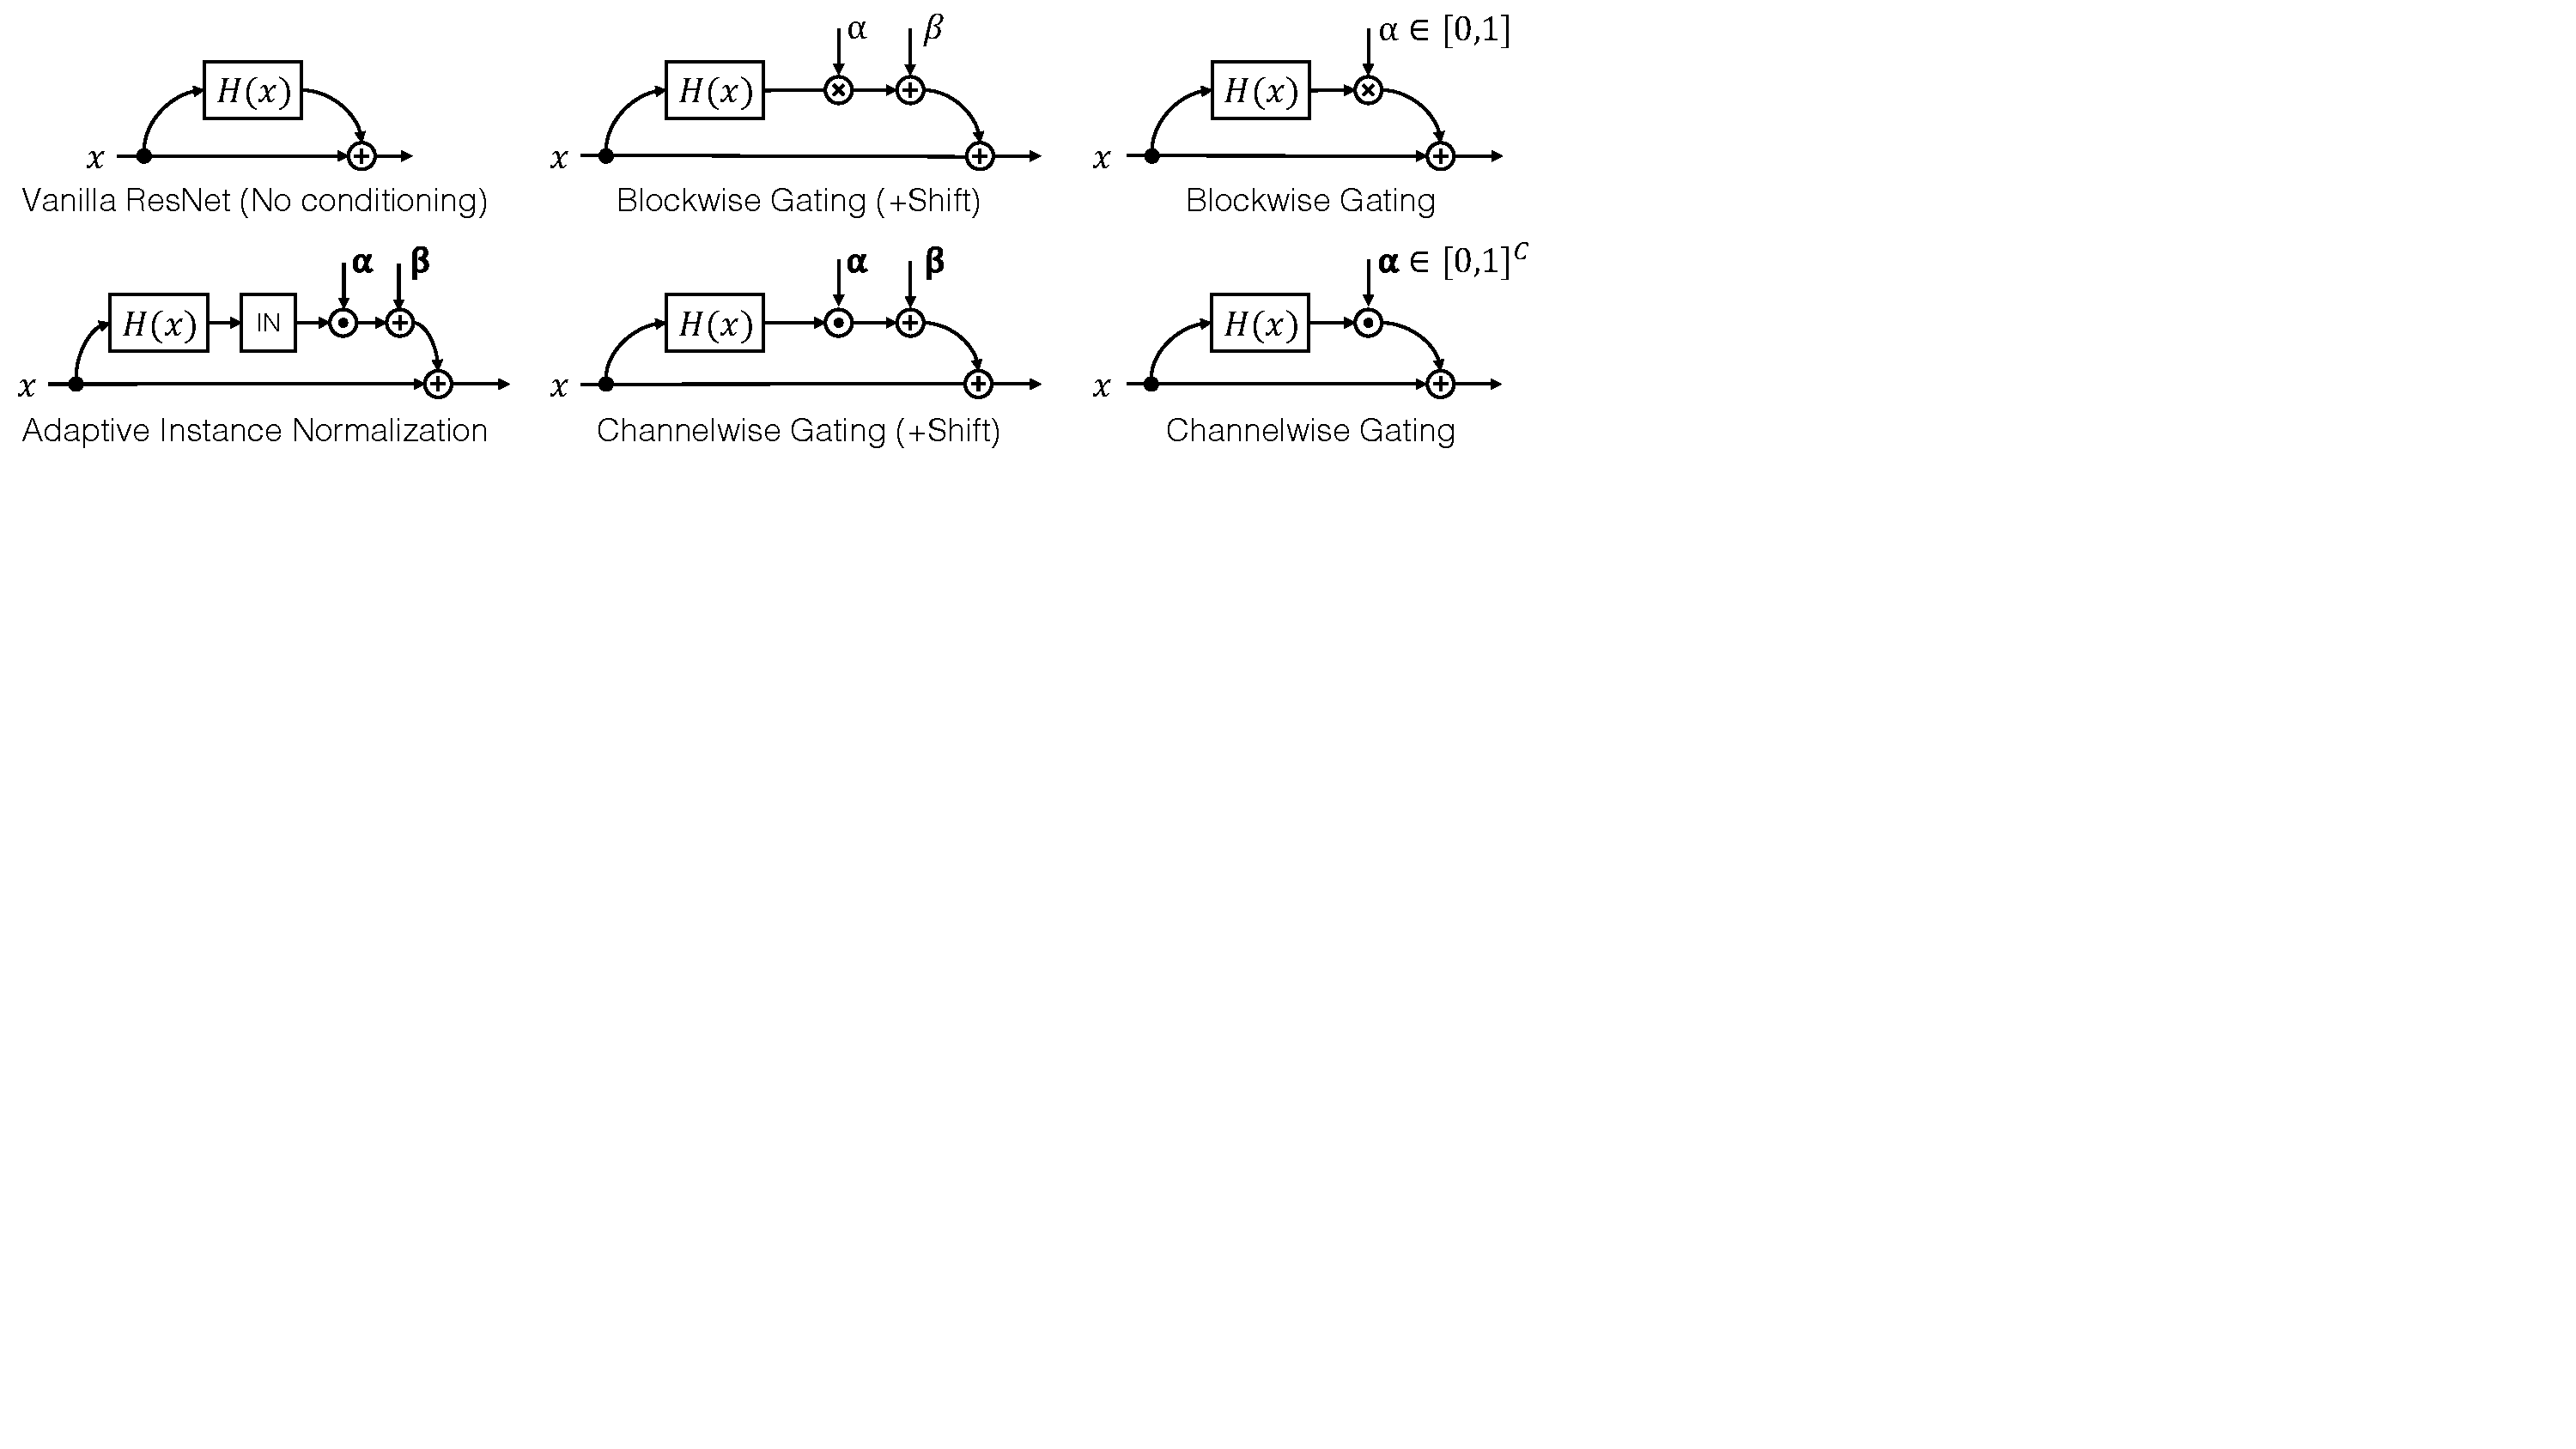
\includegraphics[width=\linewidth]{paper_images/arch_gate.pdf}
    \caption{{\bf Incorporating soft-gating into residual blocks.} \rz{Order got changed, may or may not need to add key for hadamard product} {\bf (Top-left)} A ``vanilla" residual block without gated conditioning parameters modifies signal $x$ into $x+\mathcal{H}(x)$. {\bf (Top-mid)} The full $\mathcal{H}(x)$ block is softly-gated by scalar parameter $\alpha$. {\bf (Top-right)} Each channel is softly-gated by vector parameter $\mathbf{\alpha}$. {\bf (Bot-left)} Adaptive Instance Normalization applied after the whole residual operation involves both a scaling and a bias. {\bf (Bot-mid, Bot-right)} A bias can be added to either block-wise or channel-wise gating. We find that channel-wise gating (without added bias) to empirically produces the best results.\label{fig:arch-gate} }
    % \vspace{-4mm}
\end{figure*}

\section{Related Work}
\paragraph{Mode Collapse} is a major challenge for GANs \cite{goodfellow2014generative}, where a the diversity of the generated results is limited and only a portion of the training set being utilized. Several techniques deal with this issue, the best performing among those include Spectral Normalization \cite{miyato2018spectral} which normalizes the spectral norms of the layers to stabilize training, MAD-GAN \cite{ghosh2017multi} which introduces multiple generators, BicycleGAN \cite{zhu2017toward} which reconstructs back the latent code from the generation using two cycles. MUNIT \cite{huang2018multimodal} introduces factorized latent space for content and style for producing variations.

\paragraph{Residual Networks and Gating Mechanisms} Residual Networks \cite{he2016deep} introduced a new set of architectures that enabled training of very deep networks. The incision experiments performed in \cite{veit2016residual} demonstrated that few paths were more important for particular classes and designed an adaptive residual network in \cite{veit2018adaptive} albeit they have a hard gating mechanism in contrast to our soft gating mechanism. Our approach has relation to the widely used Adaptive Instance Normalization albeit the predicted parameters are unconstrained in that situation while ours is not. Although previous work has explored the idea of gating via AdaIN in the generator but our techniques also involves using gating in the discriminator as well. FiLM \cite{perez2017film} is a gating mechanism introduced in the realm of Visual Question Answering and uses similar principles albeit gating mechanism is conditioned on the input question. Soft Gating has previously been used for Natural Language Processing in LSTMs \cite{hochreiter1997long} and GRU \cite{cho2014learning}

\paragraph{Conditioning for Image Generation}
Pix2pix \cite{isola2016image2image} introduced a set of tasks whereby the pixels of the input in a different domain corresponded to the pixels of the generated image but needed far more details such as in the case of edge to handbags generation task it needed texture strokes inside the bag as well to be able to produce high quality diverse generations. Other forms of conditioning have been introduced in \cite{wang2018video} whereby rough triangles and sparse edges are enough to generate high quality videos. We explore the situation in which the input scribble is extremely sparse and multiple classes can have very similar input scribbles for instance in the case of balls the input scribble is just the outline in the shape of a circle.

Our architecture also differs from previous art in the form of the architecture whereby all the blocks are residual including the downsampling and upsampling. Previous literature mostly used the residual blocks in the bottleneck layer of an Encoder Decoder structure. The number of channels in the networks doesn't change with the change of resolution as in the original Resnet architecture \cite{he2016deep} in order to ease the learning of the gating mechanism. 

% The seminal work by \cite{miyato2018spectral}, introduced spectral normalization which normalizes the weights of the network such that the maximum eigen value of the resulting set of weights is bounded. It helped enormously in stabilizing the training of GANs and albeit they only applied spectral normalization to the discriminator, SA-GAN \cite{zhang2018self} applied it to both the generator and discriminator and showed superior generative modeling performance over several tasks. SA-GAN further introduced the self attention layer based on the innovative transformer network and showed not only better geometric properties being modeled by the GAN but also allowing Multi-Class generations.
% The Projection Discriminator \cite{miyato2018cgans} based Conditional GANs altered the naive model of concatenating the condition provided to the discriminator via a generalized bilinear projection between the condition and the features extracted from the image thereby providing more finegrained gradients suitable for training the generator to produce class conditional and better resolution images. 
% MAD-GAN \cite{ghosh2017multi} introduced multiple generators and showed an innovative experiment whereby they mixed images from 3 classes and the 3 generators could disentangle the classes and each of the generators generated much sharper images from a particular class than a single generator with similar capacity could. 

% %moved from intro
% To combat this challenge a solution called MAD-GAN \cite{ghosh2017multi} was proposed which dealt with the issue via multiple generators whereby the discriminator distributed the modes and classes in the data distribution among the various generators. 
% Although MAD-GAN was a novel solution to deal with discontinuities in the manifold of the multi-class data distribution, the solution came with its flaws, supreme among them was the reduced scalability in the case the structure was not shared among the different classes, the generators couldn't share the initial layers' parameters and therefore was limited by GPU capacity and in practice going more than 5-6 generators was difficult. 

% In another line of papers which helped build the ideas in this paper are the research on Residual Networks \cite{he2016deep} which introduced a set of architectures which allowed extremely deep networks to be trained upto hundreds of layers which was earlier assumed to be extremely difficult because of the problem of vanishing gradients in deep networks. The residual connection allowed a unadulterated gradient backpropagation pathway which enabled training of ultra deep networks. A thorough analysis of residual networks by \cite{liao2016bridging} showed that residual networks have similar connections to unrolled recurrent neural networks without weight sharing and is very similar to how computation unfolds in human brains. Veit et al. \cite{veit2016residual} did a set of innovative incision experiments whereby they removed some blocks and allowed only the skip connection to be active in a trained Residual Network and they were able to demonstrate that even after removing some layers there a very miniscule reduction in the classification accuracy while a similar incision in a VGG network \cite{simonyan2014very} which doesn't have skip connections led to almost random outputs in the task of classification. \cite{veit2016residual} also demonstrated that residual networks behave as an ensemble of several shallower networks. \cite{veit2018adaptive} used the concepts introduced in \cite{veit2016residual} to introduce a discrete gating mechanism in deep residual networks based on the Gumbel-Softmax approximation to make the discrete decision differentiable. Their approach allowed redundant computations in the residual blocks to be reduced and to use only few of the blocks in the trained network during testing phase of the neural network. \cite{de2017modulating} introduced a technique for modulating the activations of a residual block by predicting the parameters of batch normalization which they term as Conditional Batch Normalization. In a similar vein \cite{perez2017film} also used a similar technique for modulating the activations of the various blocks conditioned on the question in a Visual Question Answering scenario.

% Gating mechanisms have generally been useful for language modeling tasks such as LSTMs \cite{Hochreiter1997LSTM} and \cite{chung2014empirical} which improved language modeling performance over vanilla RNNs. Gating also helped in the case of image recognition as demonstrated in Highway Networks \cite{srivastava2015highway} albeit it has a lot of resemblance to residual networks. 

% Image manipulation and Generation has seen huge strides in recent years with the advent of Generative Adversarial Networks \cite{goodfellow2014generative}, style transfer networks \cite{gatys2015neural} and image colorization \cite{zhang2016colorful}. iGAN \cite{zhu2016generative} was one of the first very innovative papers that introduced us to a novel technique for editing images using neural networks and preventing the edited images to fall off the natural image manifold. Pix2pix \cite{isola2016image2image} introduced a novel network based on GANs which could translate images on a plethora of datasets such as edges to handbags, semantic layout to photo realistic images and day to night. Cutting edge techniques on similar lines include \cite{wang2018video} which can translate from Video to Video such as from pose sequences to a person dancing or from semantic layouts to photorealistic road scenes. InfoGAN \cite{chen2016infogan} introduced a novel network based on GANs and Information Theoretic principles which could disentangle modes in the data distribution based on an unsupervised objective but showed poor performance in being able to disentangle modes and produce stochastic variations in the setting of pix2pix which is known to collapse to a single output for a particular input whereas ideally it should be a distribution. Bicycle GAN \cite{zhu2017toward} introduced 2 cycles which was able to produce stochastic generated outputs in the case of image to image translation. Another innovation was CycleGAN \cite{zhu2017unpaired} which allowed unpaired image to image translation as well as unpaired domain transfer which enabled several transformations which wasn't possible earlier. 

